\documentclass[12pt]{article}
\usepackage{amsmath}
\usepackage{authblk}
\usepackage[utf8]{inputenc}
\usepackage{subcaption}
\usepackage{natbib}
\usepackage{graphicx}
\usepackage{array}
\usepackage{tabularx}
\usepackage{booktabs}
\usepackage{makecell}
\usepackage{multirow}
\usepackage[table]{xcolor}% http://ctan.org/pkg/xcolor
\setlength{\parindent}{0pt}
\setlength{\parskip}{1em}
\usepackage{hyperref}
\graphicspath{ {./images/} }

\hypersetup{
    colorlinks=true,
    linkcolor=black,
    filecolor=magenta,      
    urlcolor=cyan,
}

\usepackage[a4paper,width=165mm,top=25mm,bottom=25mm]{geometry}
\title{\Huge User Manual}
\author{Eveborn L
        \and Klasson M}

%For tables from SQAP
\newcolumntype{n}{>{\hsize=0.7\hsize \raggedright\arraybackslash}X}
\newcolumntype{w}{>{\hsize=1.6\hsize \raggedright\arraybackslash}X}
\newcolumntype{a}{>{\hsize=1.2\hsize \raggedright\arraybackslash}X}
\newcolumntype{b}{>{\hsize=0.8\hsize \raggedright\arraybackslash}X}

\begin{document}

\maketitle
\setlength{\parskip}{0em}

\begin{center}

      \vfill

\includegraphics[width=\linewidth]{logo_heartbyte_transparent_v_1_1 (1)}

    \vfill
\clearpage


    \textbf{\large Current Version 2.5 [23-11-20]}
    \vspace{10mm}
    
    \emph{\large Previous Versions}
    
\begin{center}
\begin{tabular}{ | m{5em} | m{5em}| m{10em} |m{5em}| m{5em} |m{5em} |  } 
\hline
Version Number& Published Date & Description of revision & Author & Approved by \\ 
\hline
1.0 & 2020-10-13 & Document Plan and a bit about GitLab & Martin Friberg & N/A \\
\hline
2.0 & 2020-11-04 & Wrote about SCRUM and a bit about eXtreme programming. Added things to GitLab section & Martin Friberg & N/A \\ 
\hline
2.1 & 2020-11-15 & Added things to most parts of the process plan. New sections (Cross-functional teams and development) & Martin Friberg & N/A \\
\hline
2.2 & 2020-11-15 & Enhanced the sections regarding Cross-functional teams and Management team & Axel Trolme & N/A \\
\hline
2.3 & 2020-11-17 & Enhanced the section for Management & Sam Anlér & N/A \\
\hline
2.4 & 2020-11-18 & Added the section for Analysis and Testing & Max Klasson & N/A \\
\hline
2.5 & 2020-11-23 & Updated GitLab section with Kanban board info and revised the branch section & Martin Friberg & N/A \\
\hline
2.6 & 2020-11-26 & Added section for naming convention on components & Martin Friberg & N/A \\
\hline
\end{tabular}
\end{center}

\end{center}

\clearpage
    {
 
        \renewcommand{\contentsname}{Innehåll}
        \tableofcontents
    }
    
\clearpage


\setlength{\parskip}{1em}
    
    \pagebreak
    % Purpose of document
    \section{Introduction}
    In this section, the purpose for the User Manual and an introduction to the website is detailed.

\subsection{Background}

This website was created to simplify the management of multiple patients at one operation.  

\subsection{Purpose}

The purpose of this manual is to in an easy way with help of screenshots from the website describe the different views and features of the website and how they work. 

\subsection{Introduction to website}

The website is divided into three different views, the login page, an overview page and one view for a single patient. The overview page contains information for a number of patients while the single patient page is for a specific patient. The overview page and the page for a single patient can not be reached unless you logged in before.
    \pagebreak
    
   % How to monitor patients
    \section{Page views}
    In this section, the different sections of the web page is further described. As earlier described there are three, the login page, an overview page and one view for a single patient. The overview page and the page for a single patient can not be reached unless you logged in before. When logged in there is always a possibility to log about by clicking on the log out button in top right corner. 

\subsection{Login}
    \begin{center}
    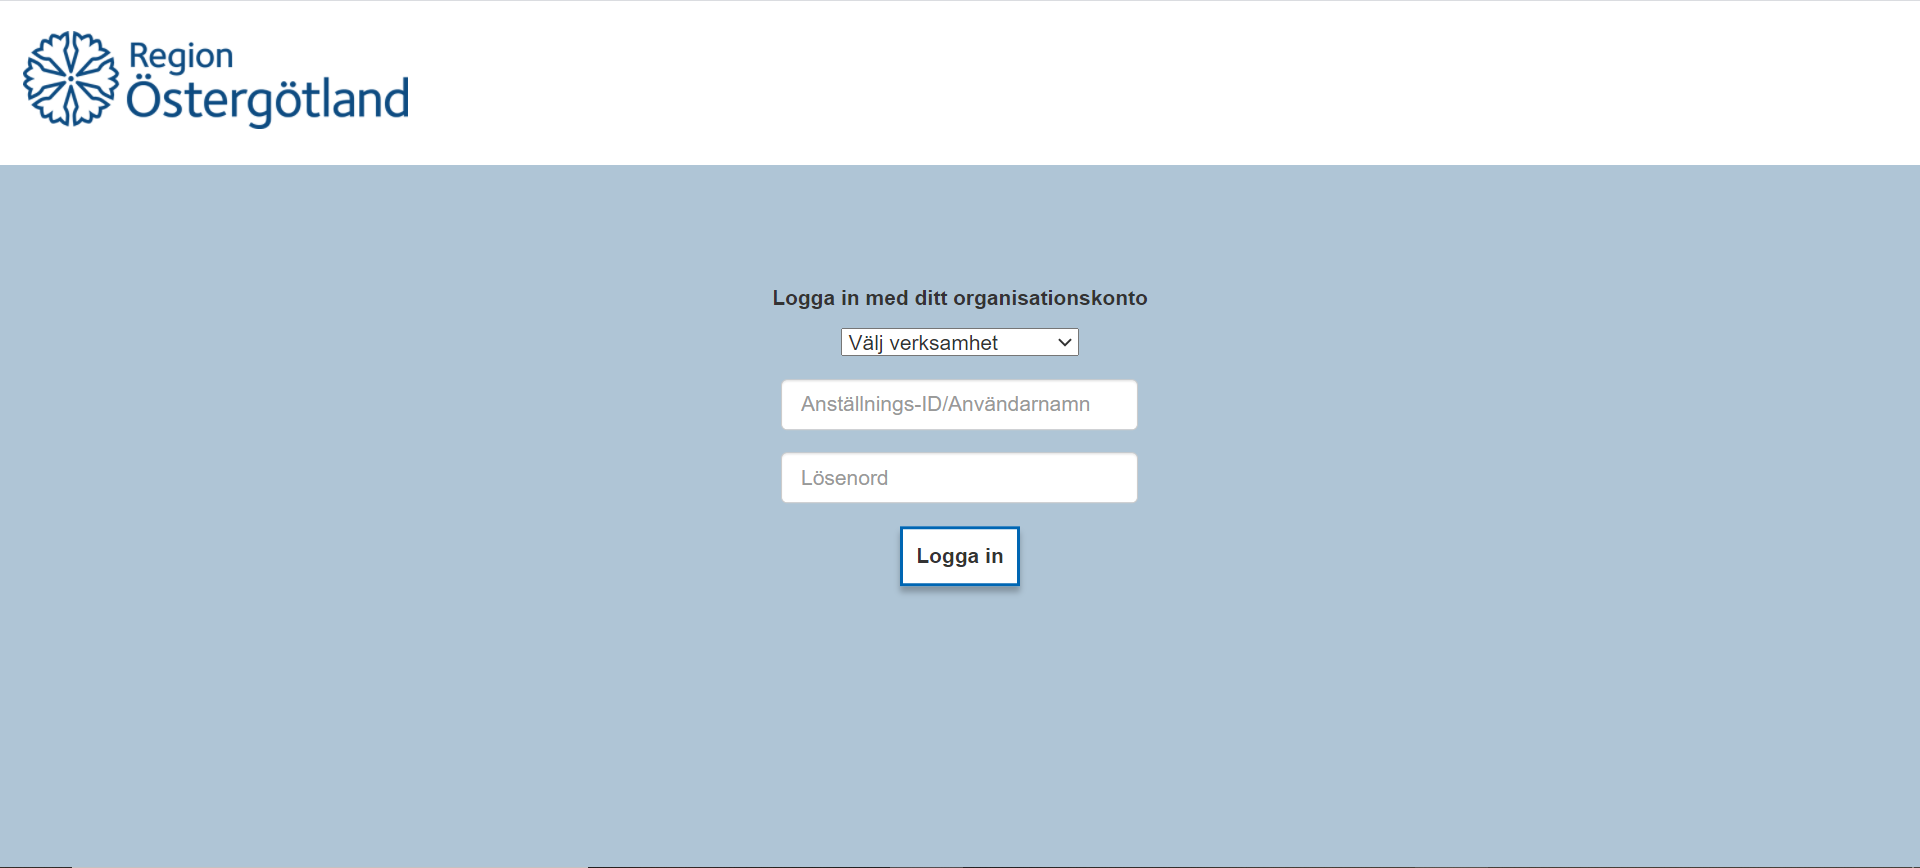
\includegraphics[width=\linewidth]{images/Login_Image.png}
    \captionof{figure}{Login}
    \label{fig:figures}
\end{center}
First page shown when signing in to the system. Start by selecting the operation (verksamhet) and then log in with the employment-ID or username and then enter a password. Successful login leads to the “Mina patienter” page.

\pagebreak
\subsection{Overview}
    In this section, the overview view is described further. The overview view is where you go after being logged in.

\subsubsection{My patients}
    \begin{center}
    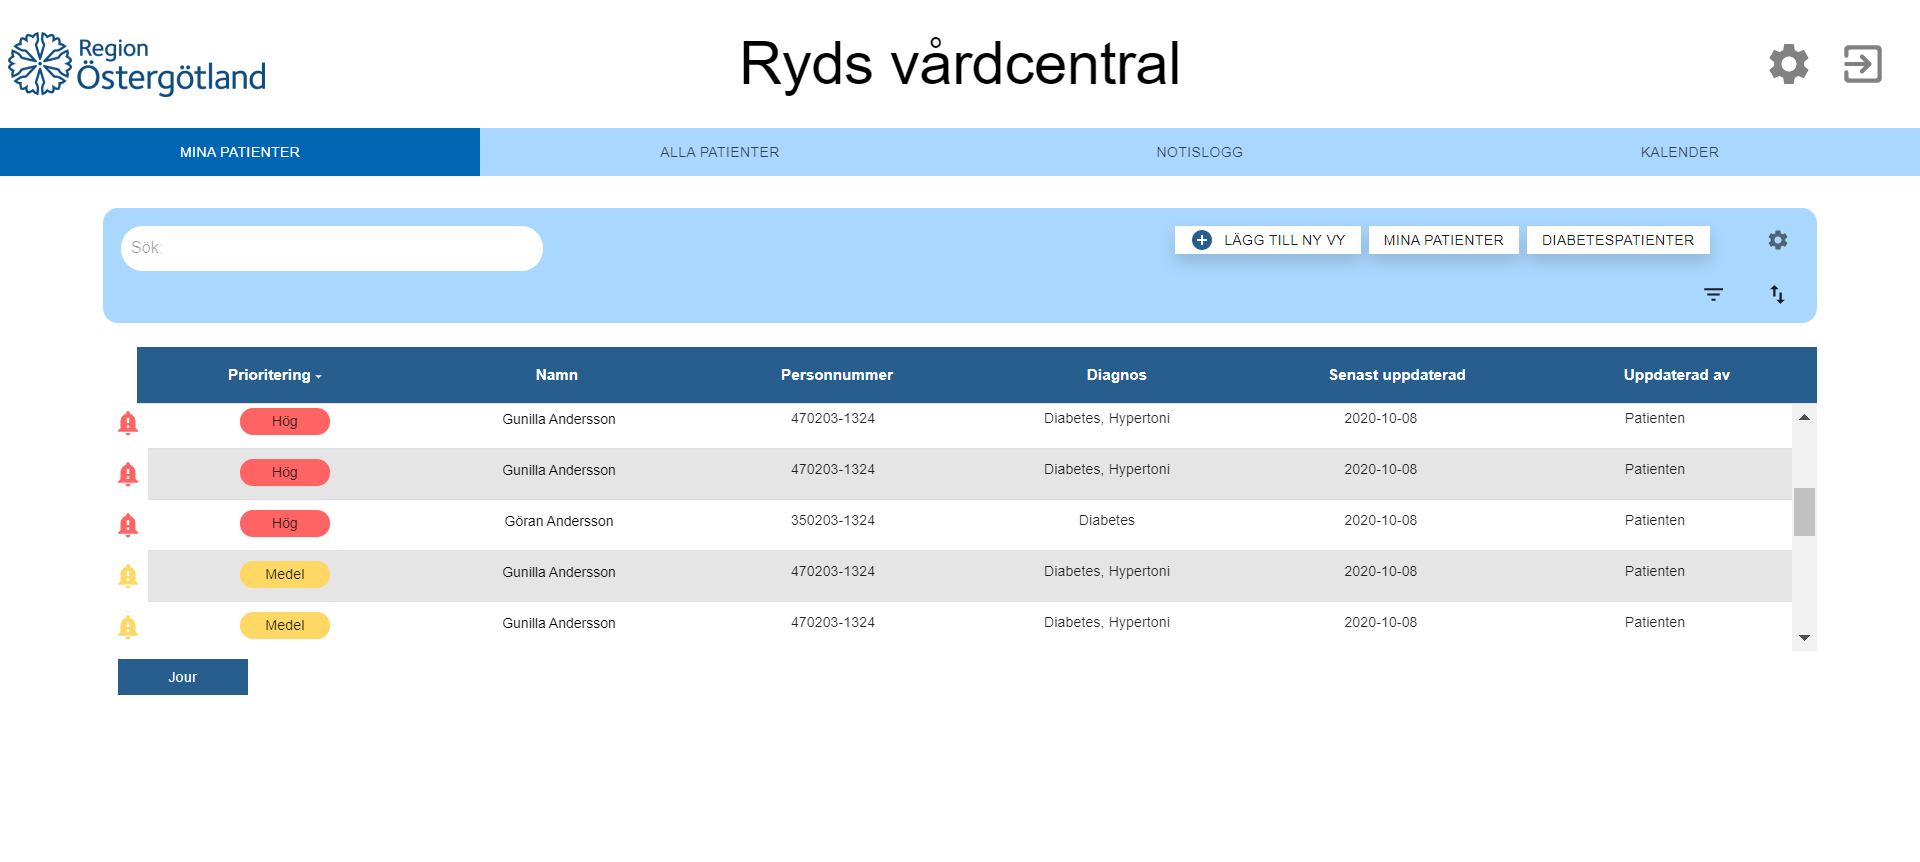
\includegraphics[width=\linewidth]{images/My_patiens_image.png}
    \captionof{figure}{My patients}
    \label{fig:figures}
\end{center}
Shows a table of all patients in the system connected to the operation (verksamhet) you are logged in to. There is an possibility to search for specific patients, filter, sort and modify the list the list. To see more about a specific patient the patients name is clicked and you are moved to the single patient's page.

By clicking on the "Jour" button at the bottom of the page a list of the doctors on call is shown, with telephone number and name.

To modify the list the gear symbol at the top right in the search bar is clicked and then in the pop-up window which appears choose the attributes wanted by ticking the associated checkbox and clicking on "Spara" (save).

To sort the list after a specific attribute the two arrows at the mid right in the search bar is clicked and then clicking on the wished attribute to sort the list after. 

To filter the table the reverse pyramid of lines at the bottom right in the search bar is clicked. A pop-up window appears, where the filters are chosen. The pop-up window looks exactly the same as the one for creating a new view which is further described below. 

There are a ability to add new views and save filters, for example one for women over 60 which has diabetes. It is possible to add up to 7 save filters. To add a filter you start by clicking "+Lägg till ny vy". A pop-up window then appears which is further described below. 

When a filter or view is active a button named "Rensa filter" shows up. By clicking on it the active filter or view is removed. 
\\

\begin{center}
    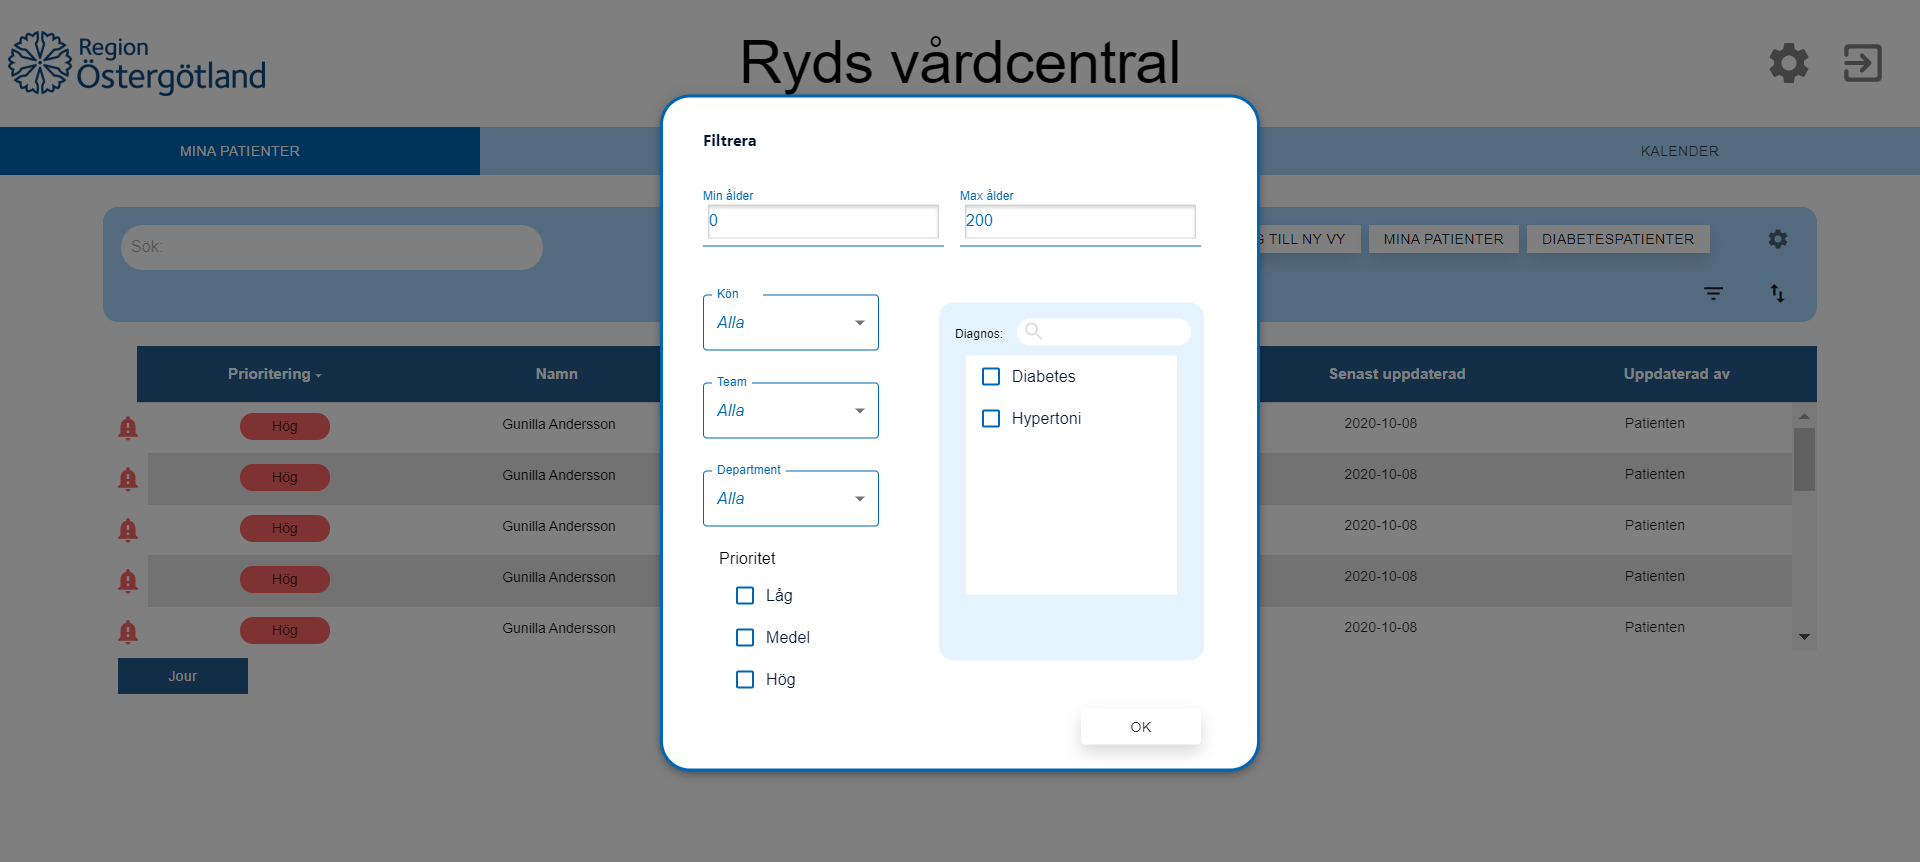
\includegraphics[width=\linewidth]{images/Add_new_view_image.png}
    \captionof{figure}{Add view}
    \label{fig:figures}
\end{center}
The pop-up window which appears when creating a new view consists of a number of attributes which can be set according to preferences. To move on click on the button "OK". To quit, just click somewhere outside the pop-up window.
\\
\begin{center}
    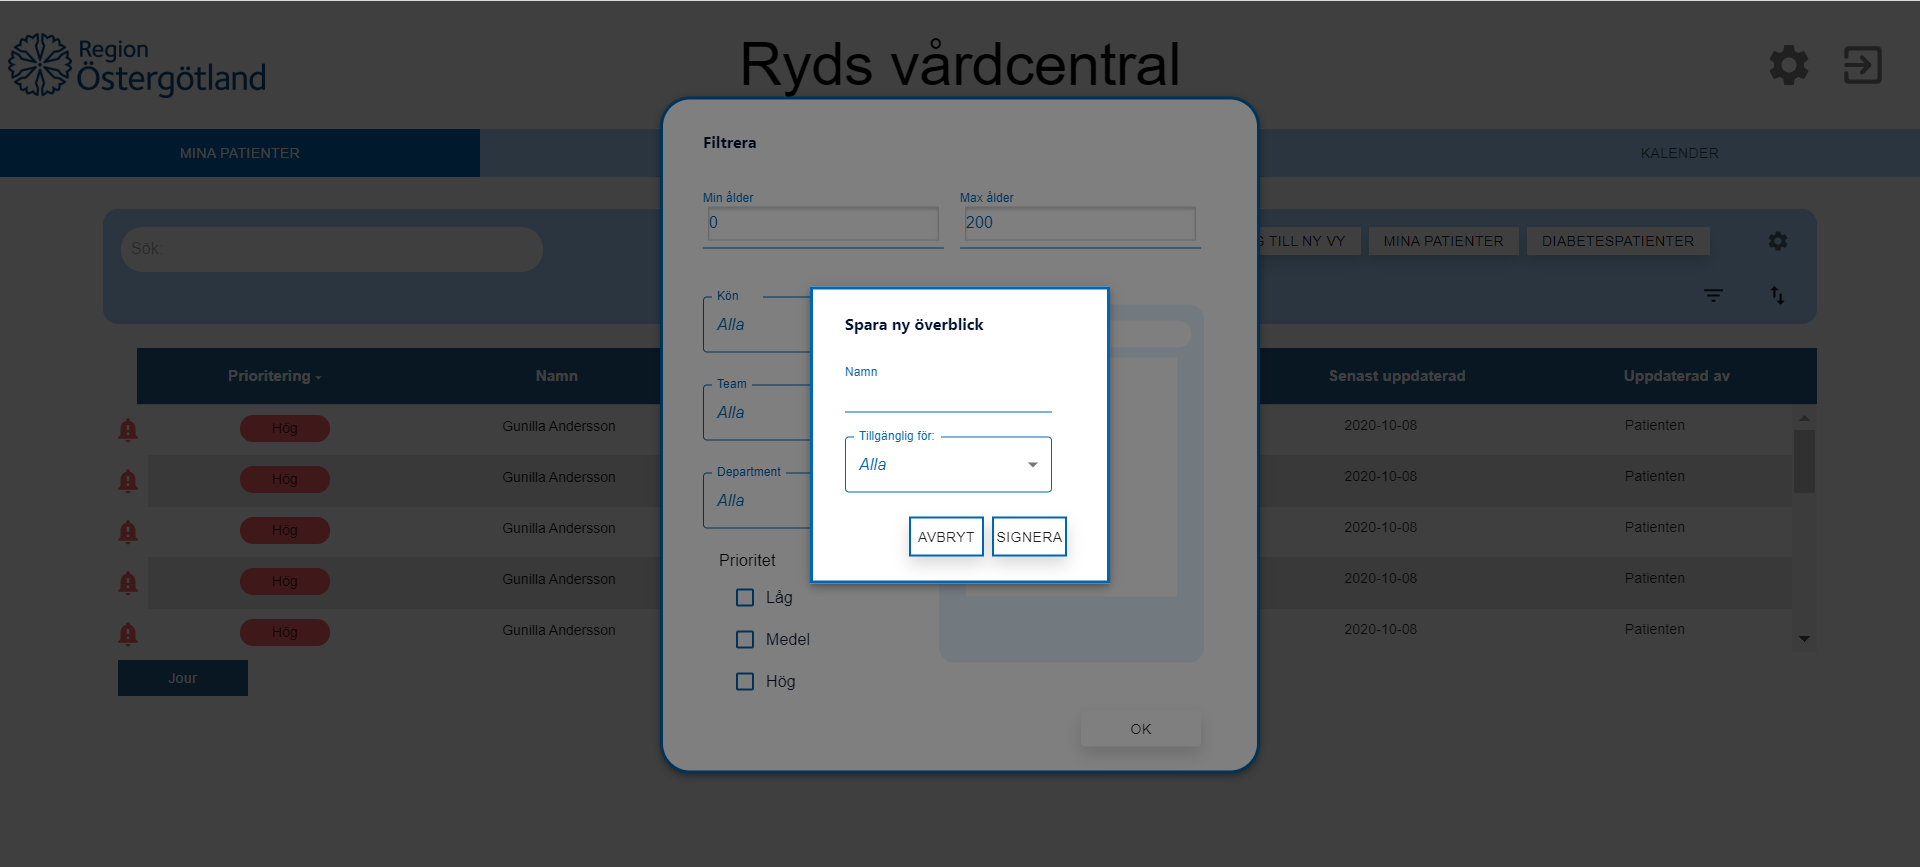
\includegraphics[width=\linewidth]{images/Save_new_view_image.png}
    \captionof{figure}{Save view}
    \label{fig:figures}
\end{center}
When preferences are chosen and clicked "OK" in the pop-up window another pop-up window appears with some further info that needs to be filled in. To finish click the "Kvittera" button. If clicking the "Avbryt" button you are moved back to the previous pop-up window.
\\


\subsubsection{All patients}
All patients is exactly the same as my patients except that it contains all patients.

\subsubsection{Notice log}
\begin{center}
    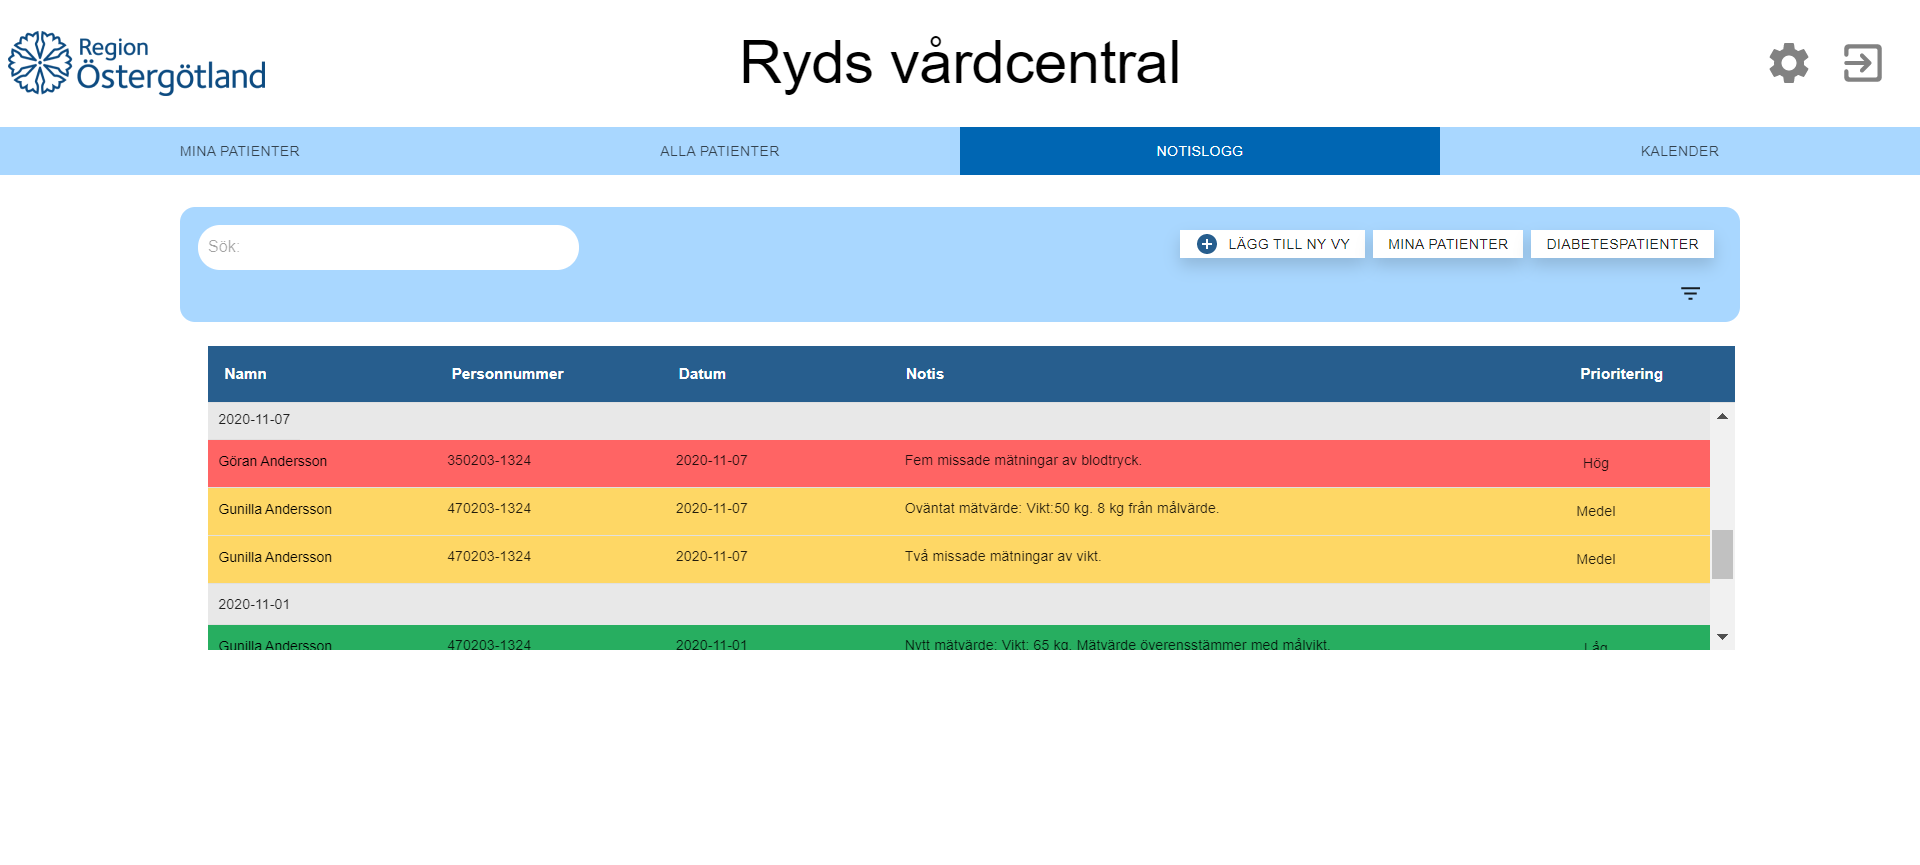
\includegraphics[width=\linewidth]{images/Notice_log_image.png}
    \captionof{figure}{Notice log}
    \label{fig:figures}
\end{center}
All the activities that happen are gathered in this notification log with a prioritization of how important the notification is to be handled. For example, if a measured value is taken with a large deviation from the average value, this should indicate a high prioritized notification. 
Same filter/search box as in “Mina patienter” and “Alla patienter”.
\\

\subsubsection{Calendar}
\begin{center}
    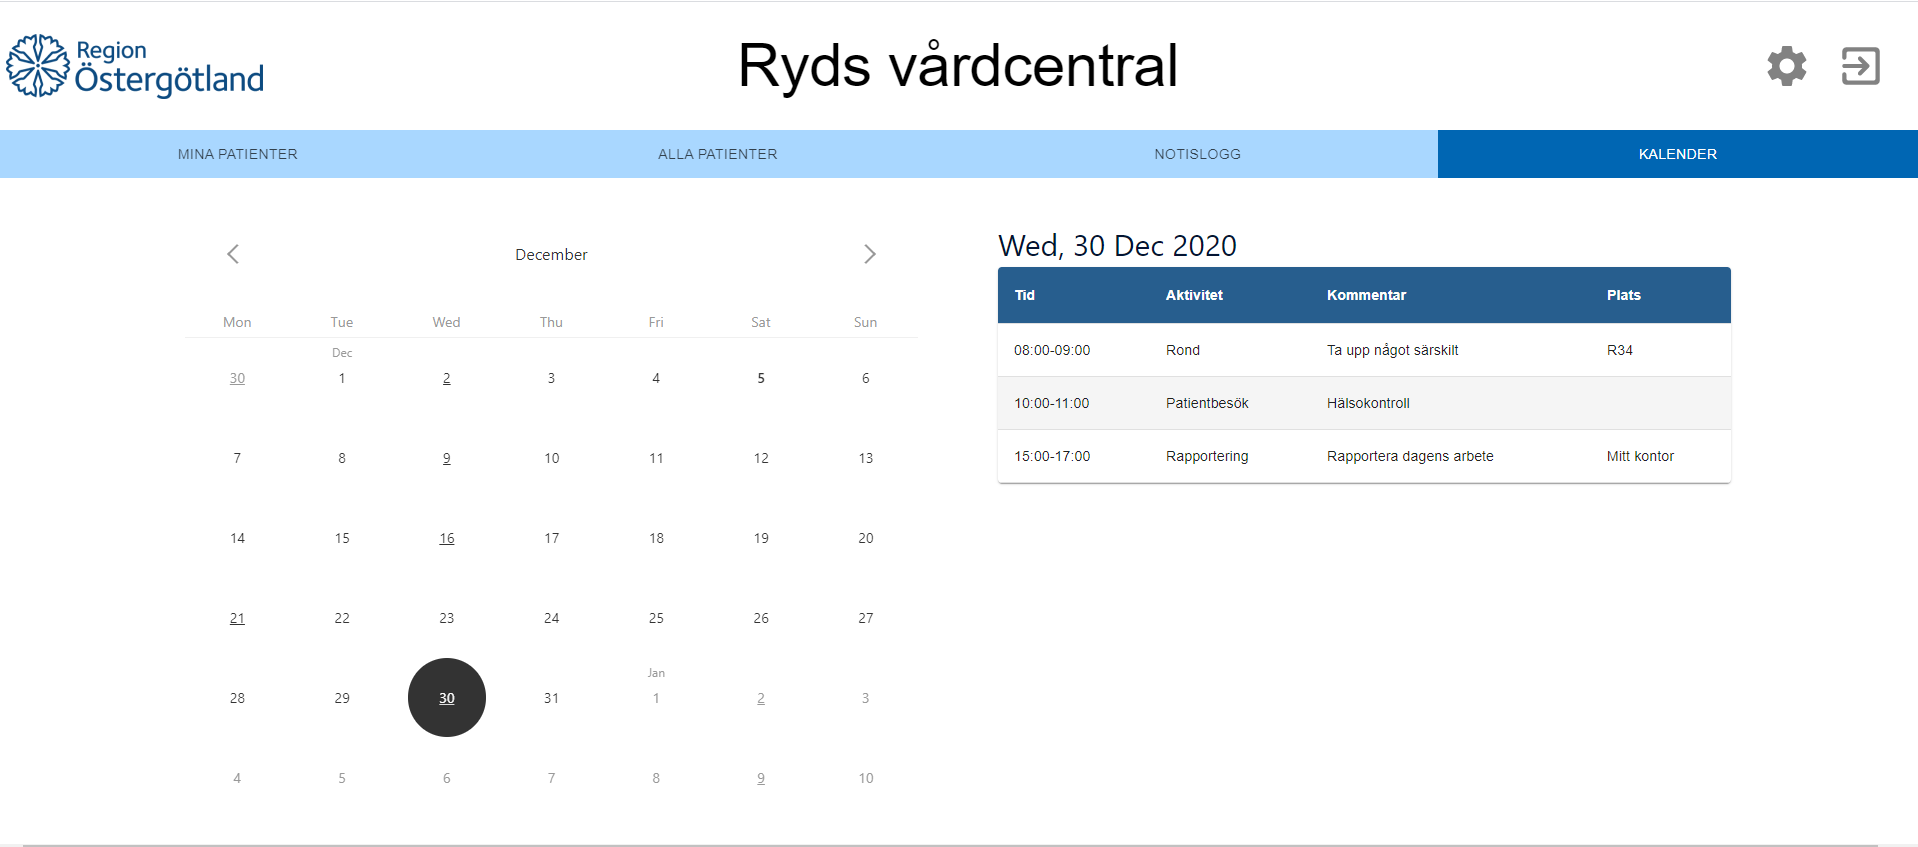
\includegraphics[width=\linewidth]{images/Calender_overview_patient.png}
    \captionof{figure}{Calendar}
    \label{fig:figures}
\end{center}
Displays a calendar view over a month. When interacting with a specific day in the calendar the booked activities are displayed in a view in a table next to it. All the upcoming activities are also shown in the table that you can scroll. By default, the current day is displayed.
\\

\pagebreak
\subsection{Single patient}
    In this section the views for a single patient is detailed. It is as earlier described by clicking on a specific patient in either my patients list or all patients list. To go back to the overview the house button which is displayed next to the patients name is clicked. 

\subsubsection{Overview}
\begin{center}
    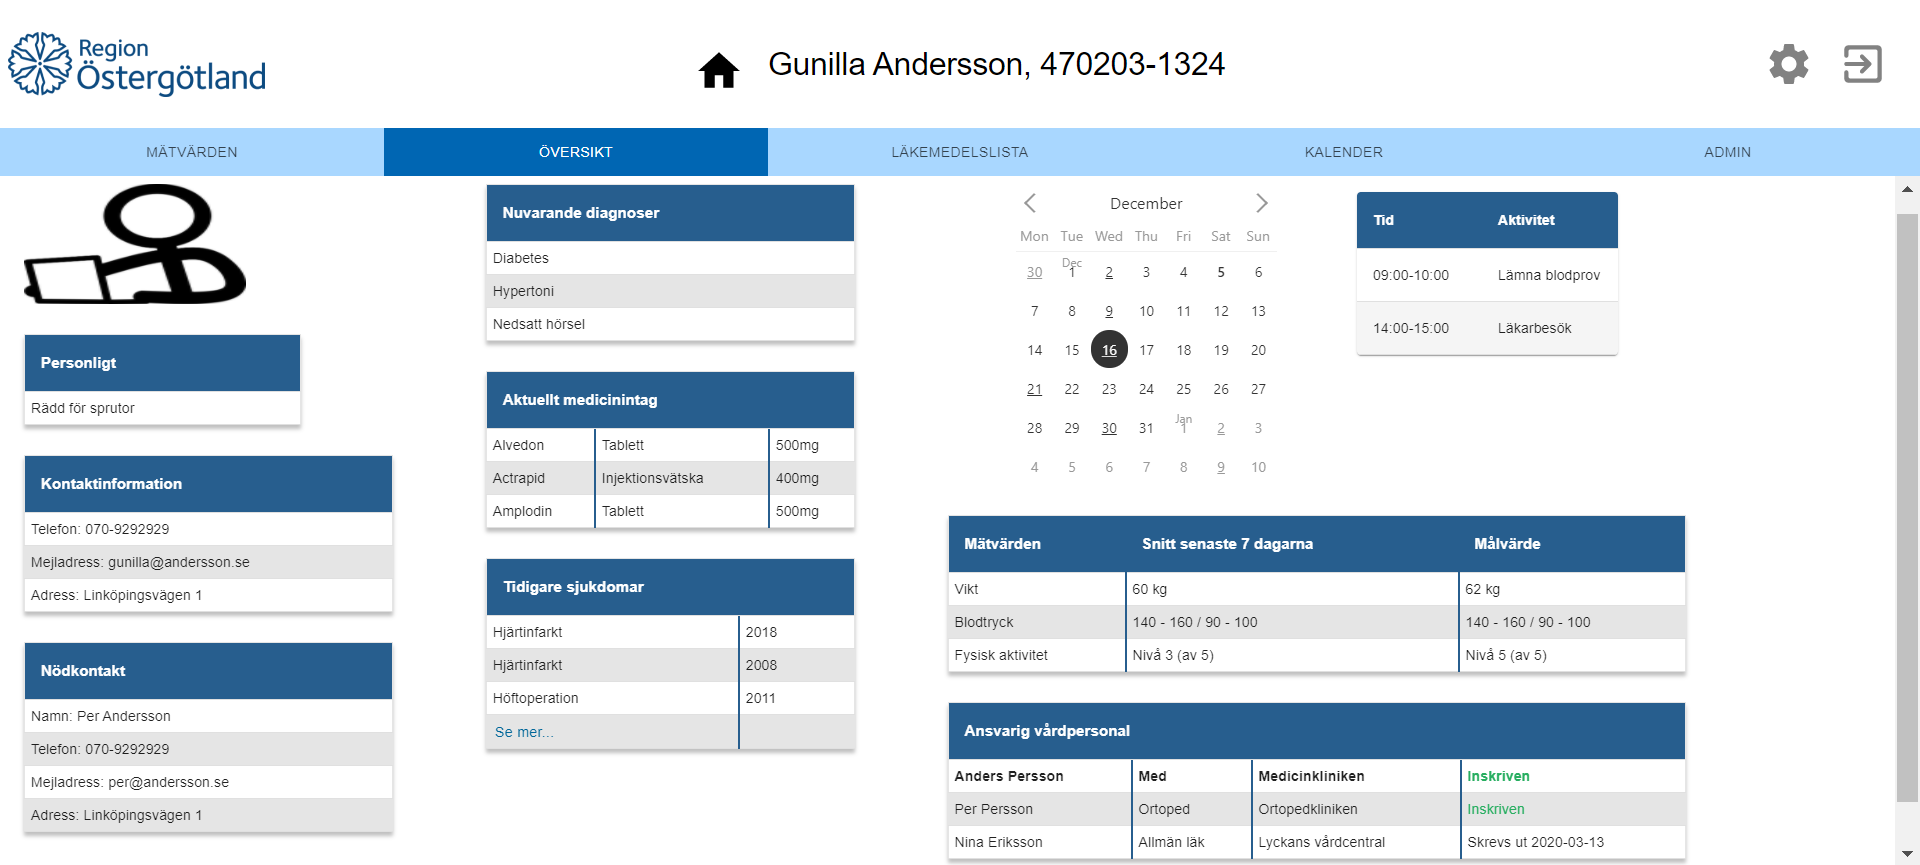
\includegraphics[width=\linewidth]{images/single_patient_overview_image.png}
    \captionof{figure}{Overview single patient}
    \label{fig:figures}
\end{center}
Information about the specific patient with contact information and emergency contact. Shows current diagnoses, current medication intake, average of current measurement values, previous diagnoses and caregivers and staff who handle the patient. Picture of the specific patient. A smaller calendar of the one found in "/patient/calendar" exists as well.

The tables length is adapted to the number of diagnoses, medications, measurements, responsible staff members. 

Table of “tidigare sjukdomar” is shown with a maximum of 4 rows with the see more text included. When pressing see more, the table expands in length and shows the rest of the information.

\subsubsection{Measurements}
    \begin{center}
    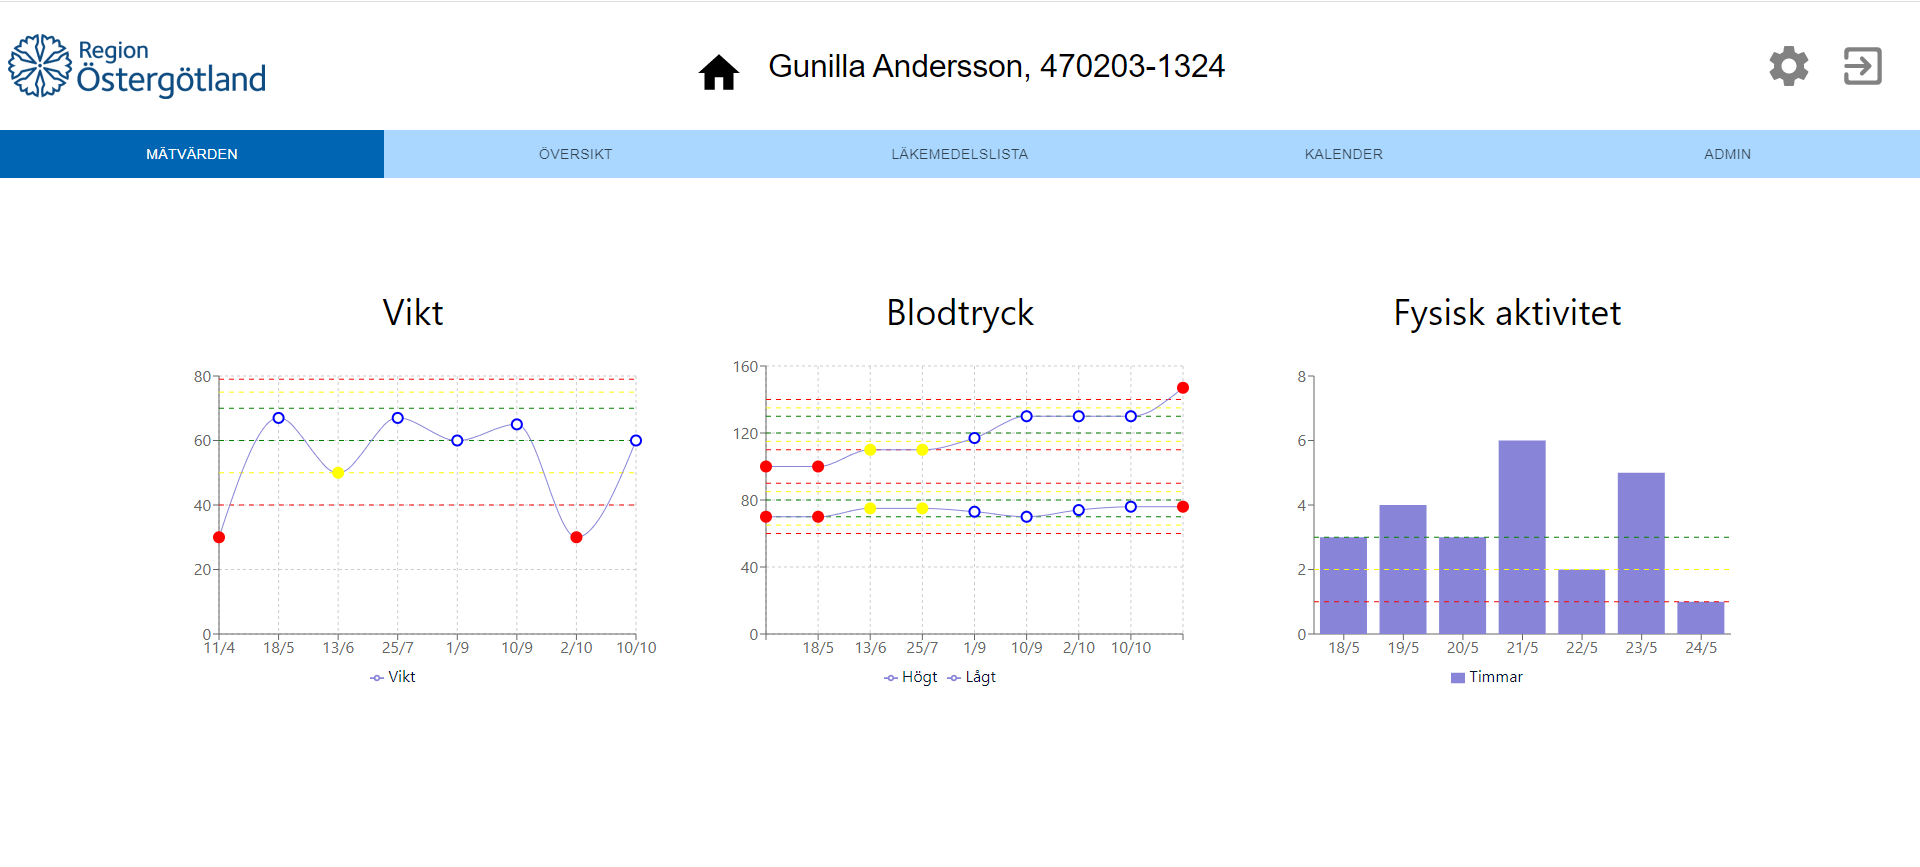
\includegraphics[width=\linewidth]{images/single_patient_measurement_overview_image.png}
    \captionof{figure}{Measurement - overview }
    \label{fig:figures}
\end{center}
All the current measurements for the specific patient are displayed in graphs. In the graph a target range is displayed but also intervals of when a red or yellow warning should be triggered. Measurement points are also seen and if they are outside the allowed references, they become red or yellow depending on severeness. By clicking on a graph you move to the specific measurement were more info and options are displayed
\\

\begin{center}
    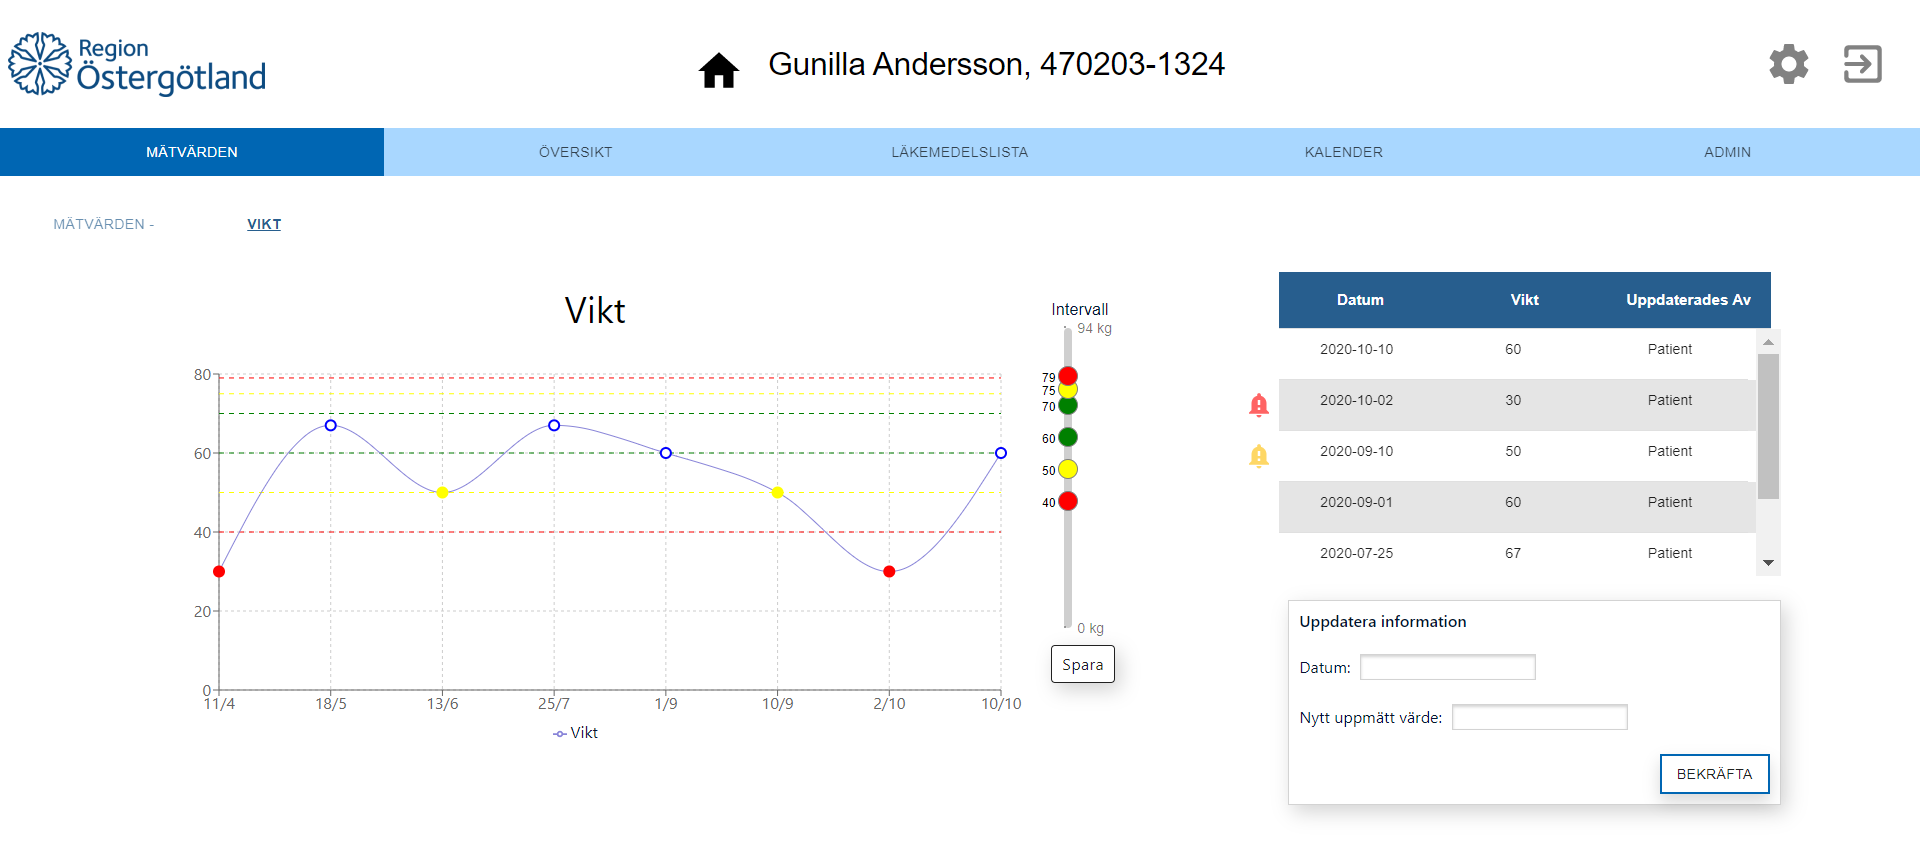
\includegraphics[width=\linewidth]{images/single_patient_weight_measurements_image.png}
    \captionof{figure}{Measurement - single page}
    \label{fig:figures}
\end{center}
On the specific page for a single measurement page, the graph works exactly like before. 

There is also a table at the page were it is possible to click on the notifications for handle the value. When clicking on the notification a pop-up window appears which is described further later. 

----------
\newline
Not fully implemented: 
For admins it is possible to change the reference ranges by moving the green, yellow and red dots displayed to the right of the graph and then click "Spara" (Save). The green dots corresponds to the target value, the yellow to severeness level yellow and the red to severeness level red. 

It is possible to add a new value by filling in the forms "Uppdatera information". Add a date and measure and click on the "Bekräfta" button.
\newline
---------

All the different subpages for specific measurements looks the same, except for that the number of target ranges and reference ranges could vary, for example blood pressure has two, one for systolic pressure and one for dystolic pressure.
\\

\begin{center}
    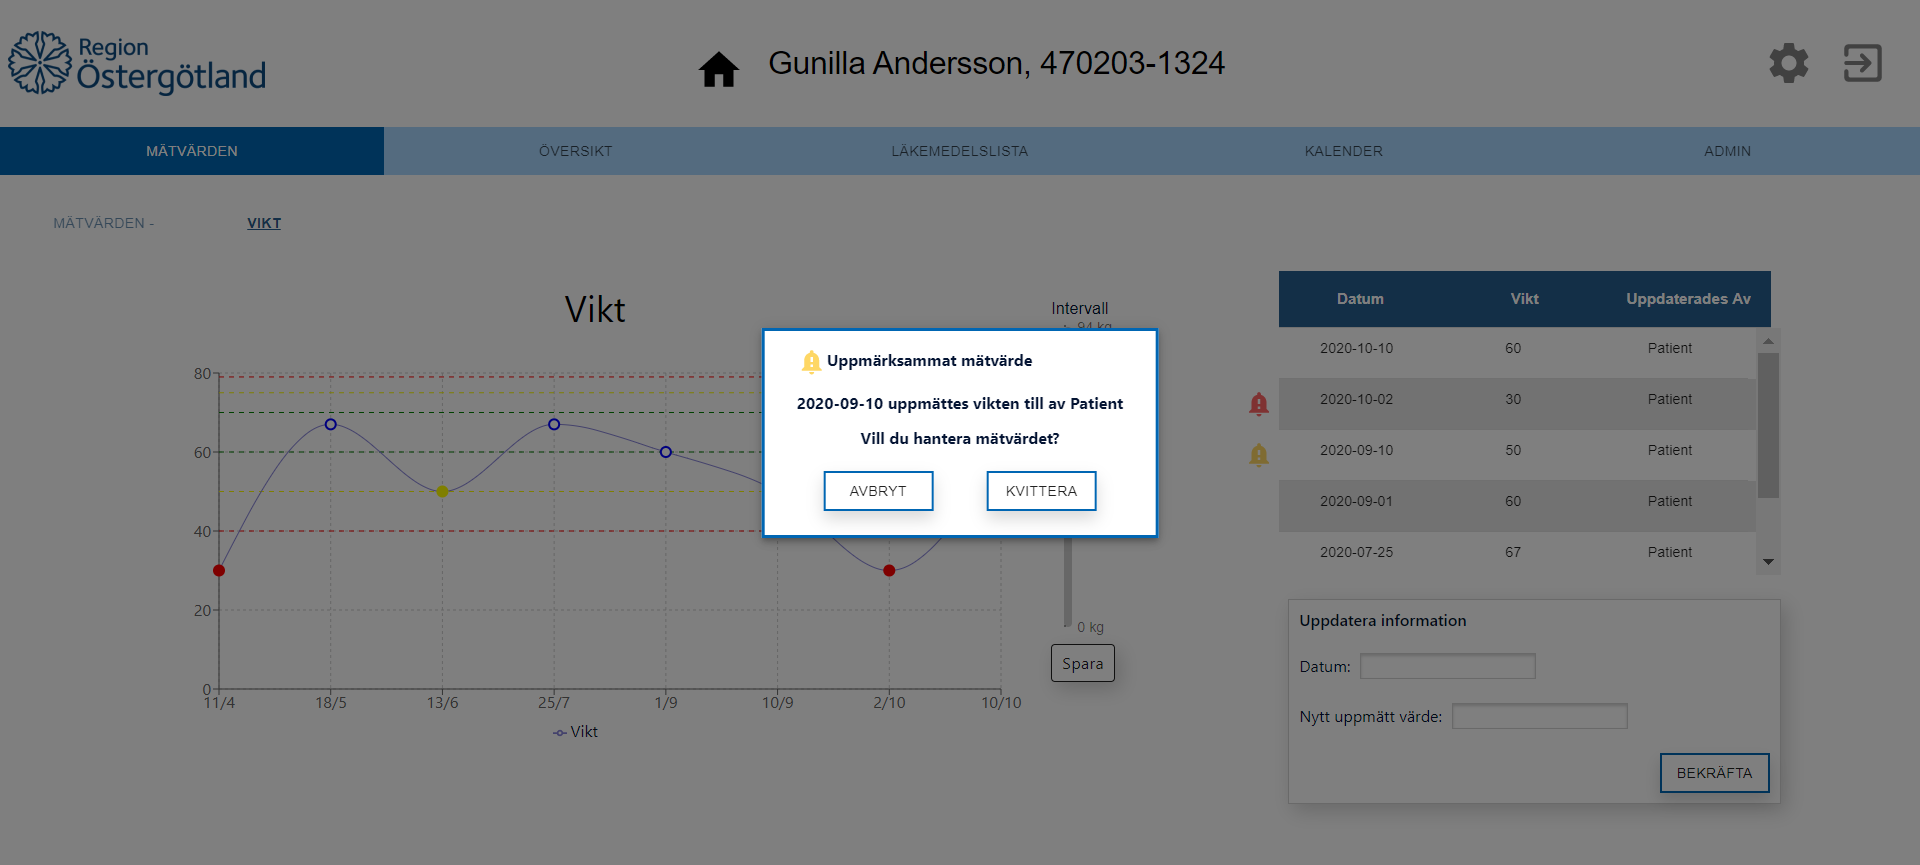
\includegraphics[width=\linewidth]{images/single_patient_weight_measurements_handle1_image.png}
    \captionof{figure}{Measurement - handle change 1 }
    \label{fig:figures}
\end{center}
When clicking on a notification a pop-up window appears with two options, "Avbryt" and "Kvittera". By clicking on "Avbryt" the pop-up window shuts down and nothing happen. By clicking on "Kvittera" another pop-up appears which is described below.
\\

\begin{center}
    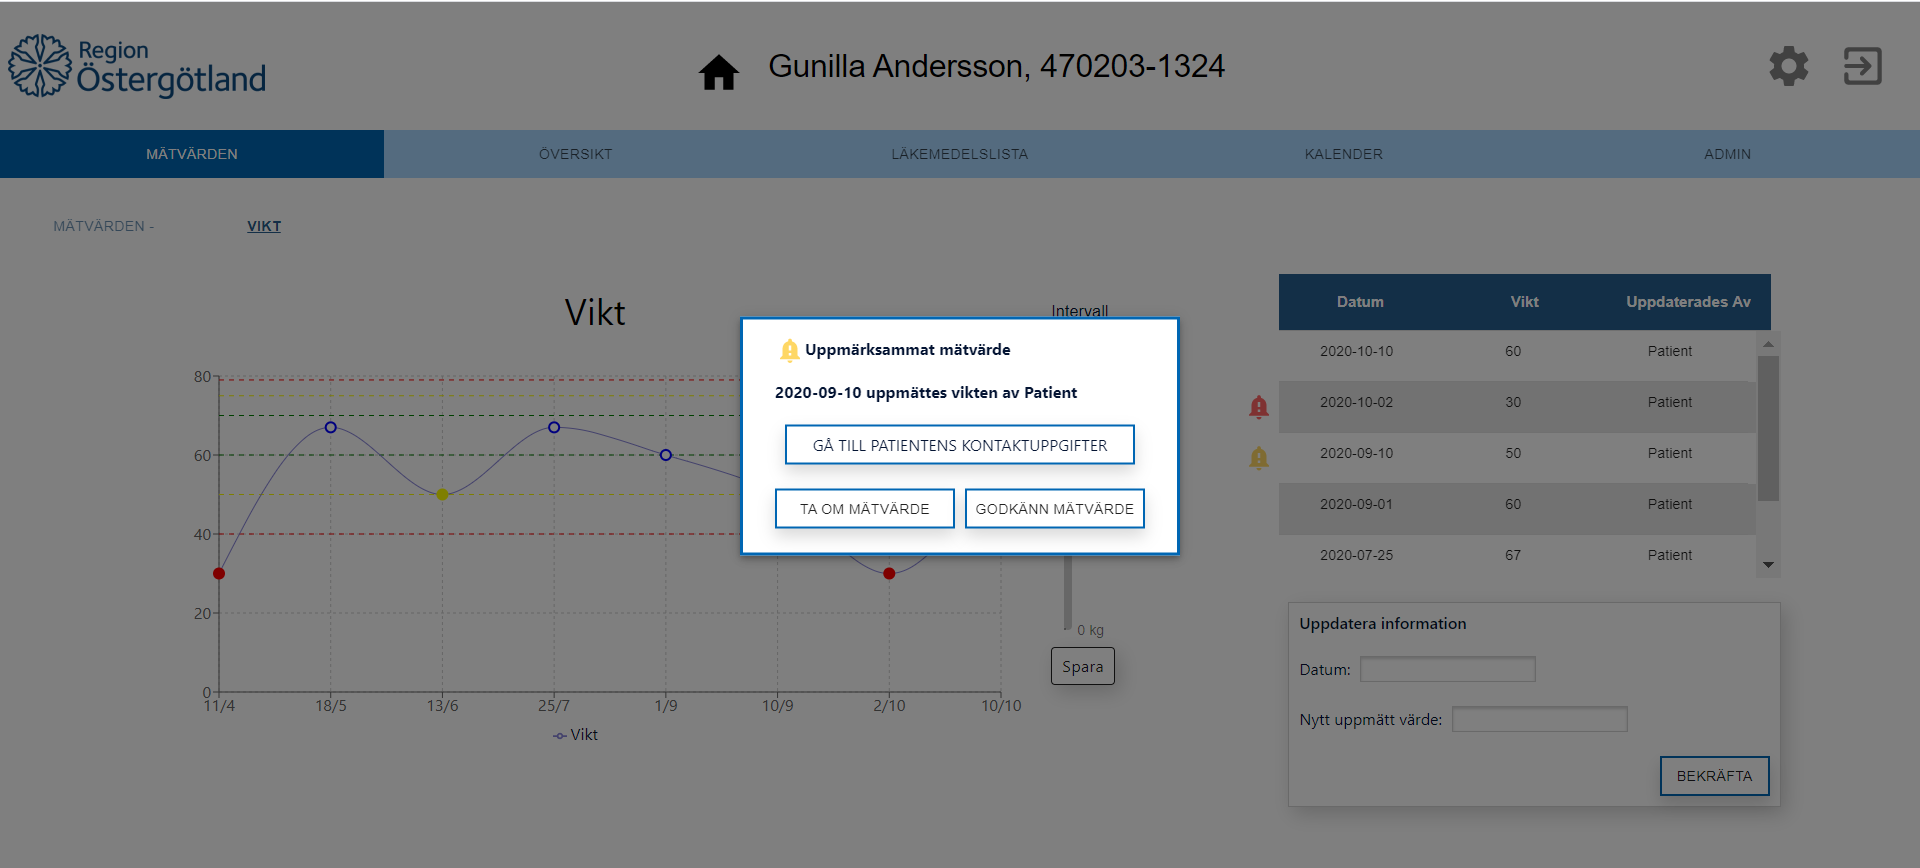
\includegraphics[width=\linewidth]{images/single_patient_weight_measurements_handle2_image.png}
    \captionof{figure}{Measurement - handle change 2 }
    \label{fig:figures}
\end{center}
If clicked on the "Kvittera" button there is now three alternatives. By clicking on "Gå till patientens kontaktuppgifter" you are moved to "patient/overview". By clicking on "Ta om mätvärde" a request is sent to the patient to retake the measured value. By clicking on "Acceptera mätvärde" the notification is taken away.
\\

\subsubsection{Medication list}
\begin{center}
    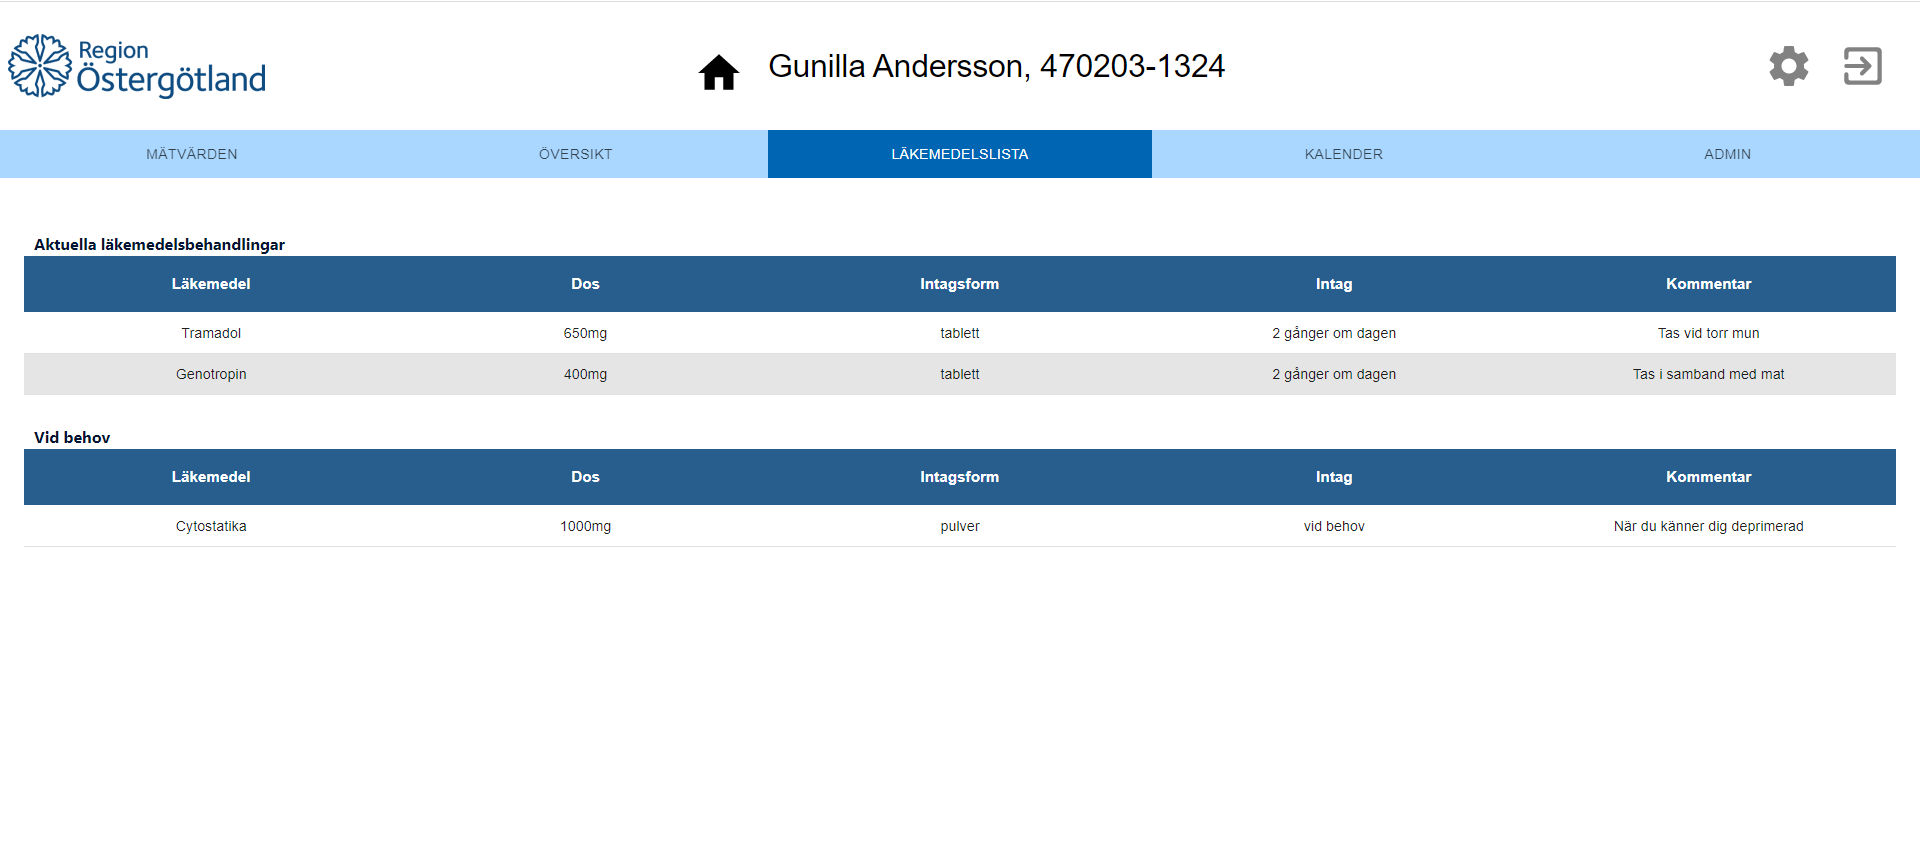
\includegraphics[width=\linewidth]{images/single_patient_medications_image.png}
    \captionof{figure}{Medications}
    \label{fig:figures}
\end{center}
Table of medicines that shows current/relevant medication intake for a specific patient and a table of medicines that a specific patient can take if necessary.
\\

\subsubsection{Calendar}
\begin{center}
    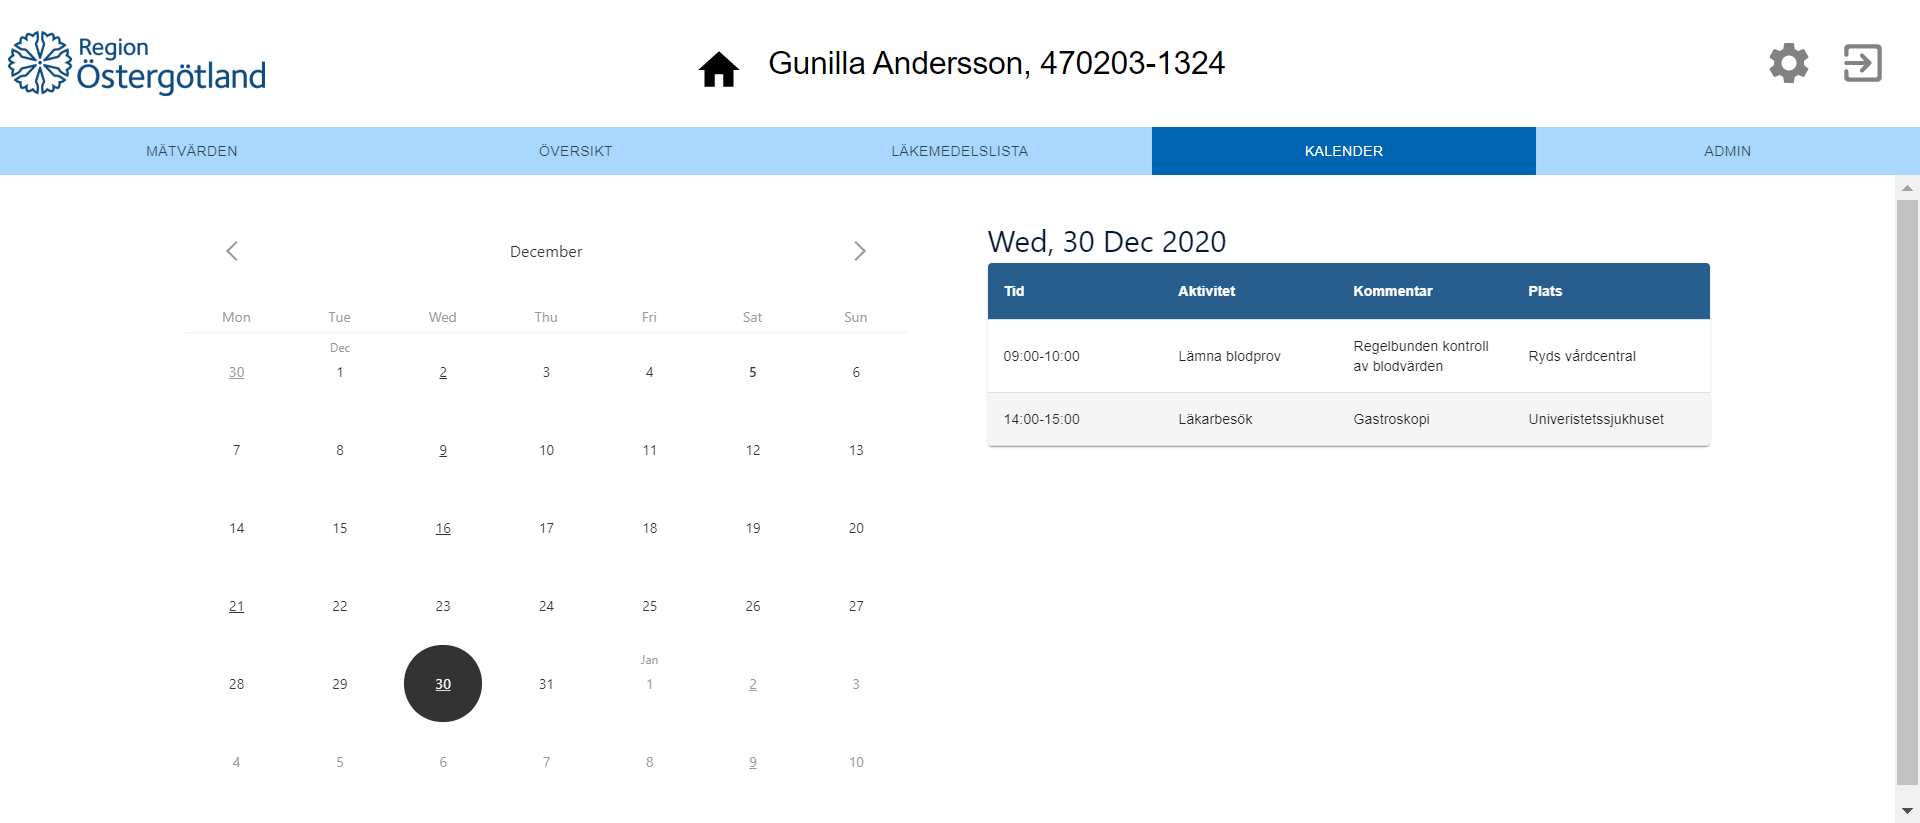
\includegraphics[width=\linewidth]{images/single_patient_calendar_image.png}
    \captionof{figure}{Calendar}
    \label{fig:figures}
\end{center}
As the calendar for all patients but this on does only display the specific patients calendar events.
\\

\subsubsection{Admin}
\begin{center}[h]
    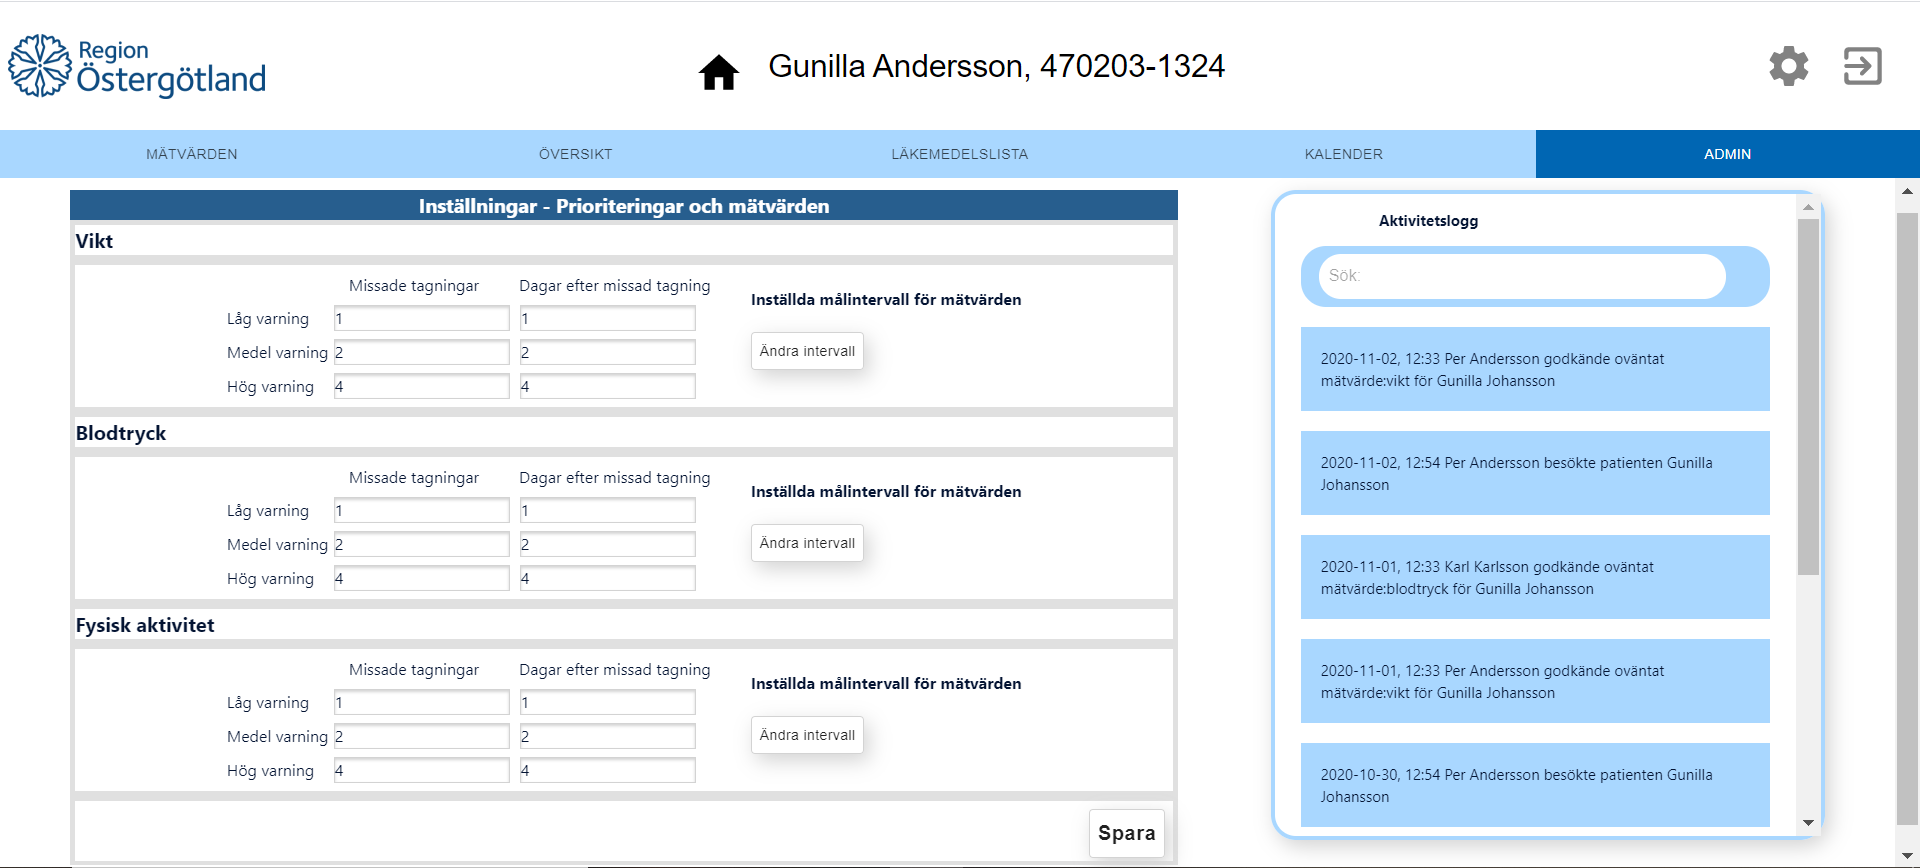
\includegraphics[width=\linewidth]{images/single_patient_admin_image.png}
    \captionof{figure}{Admin}
    \label{fig:figures}
\end{center}
Page only visible for admins. 
Inställningar Prioriteringar Mätvärden:
Set the settings for notifications for the patient measurements. The notifications are rendered by two things, either a measurement which is outside the reference ranges or that the patient have missed to report measurements. 

For changing when a warning should be rendered for missing a measurement, you change in the form for the measurement type and either days without measurement or number of expected measurements not reported, and then click on the "Spara" button at the bottom of the page. 

For changing the target ranges and reference ranges you press “Ändra intervall” and are directed to the measurement page where you can change the interval while seeing the graph at the same time. 

Aktivitetslogg: 
Shows all the activity that happens on a patient specific page. All activities is logged for the patient's integrity.
Not fully implemented: 
The search function. 

\\

    
    \pagebreak
    
\end{document}